\documentclass[12pt,letterpaper,notitlepage]{article}

\usepackage{epsfig,amsmath,amssymb,cite,color,multirow,ulem,bm}

\usepackage{graphicx,wasysym}
\usepackage{hyperref}
\usepackage{tabulary}

\usepackage{pdfpages}
\usepackage{xcolor}

\newcolumntype{K}[1]{>{\centering\arraybackslash}p{#1}}

\makeatletter
\newcommand{\thickhline}{%
    \noalign {\ifnum 0=`}\fi \hrule height 1pt
    \futurelet \reserved@a \@xhline
}
\newcolumntype{"}{@{\hskip\tabcolsep\vrule width 1pt\hskip\tabcolsep}}

\newcommand{\listintertext}{\@ifstar\listintertext@\listintertext@@}
\newcommand{\listintertext@}[1]{% \listintertext*{#1}
  \hspace*{-\@totalleftmargin}#1}
\newcommand{\listintertext@@}[1]{% \listintertext{#1}
  \hspace{-\leftmargin}#1}
\makeatother

\oddsidemargin 0cm
\evensidemargin 0cm
\marginparwidth 68pt
\marginparsep 10pt
\topmargin 0cm
\headheight 0pt
\headsep 0pt
\footskip 30pt
\textheight 22cm
\textwidth 16.5cm
\columnsep 10pt
\columnseprule 0pt

\newcommand{\tev}{\,\, \mathrm{TeV}}
\newcommand{\gev}{\,\, \mathrm{GeV}}
\newcommand{\mev}{\,\, \mathrm{MeV}}



\begin{document}

\begin{center}
\LARGE Singlet-triplet fermion dark matter\\
\Large LLP processes
\end{center}

\vspace{1.0cm}
\begin{abstract}
\vspace{0.2cm}\noindent
This file contains a list of the processes which are expected to give interesting LLP signatures in our model \cite{Filimonova:2018qdc}, possible backgrounds and signal features.
\end{abstract}

\section{Two displaced leptons}

The production goes trough Z-boson, leading to a signature with two displaced leptons of the opposite sign (Fig. \ref{fig:2displaced_diagram}). The displacement is caused by the mixing angle suppression $\theta \approx \mu/(m_T - m_S)$, the mass splitting between the charged and the light neutral states is $\Delta m_{c \ell} = 15-30 \text{ GeV}$. The lifetime of the charged state varies in the range $\c \tau_+ \simeq 0-1.5(4) \text{ cm}$ in the scalar(pseudo-scalar) scenario and the portal coupling is $\mu/v \lesssim 3\times 10^{-5}\ (3\times 10^{-4})$ in the scalar (pseudo-scalar) model.

\subsection{Main backgrounds expected}

\begin{itemize}

\item 2015 CMS $e-\mu$-search for the opposite sign leptons with large impact parameters $d_0= 0.02 - 2 \text{ cm}$, $\c \tau_{\tilde{t}}=10^{-2}-10^2 \text{ cm}$ \cite{Khachatryan:2014mea}: HF states with $\tau \simeq 0.05 \text{ cm/c}$ and $Z \rightarrow \tau \tau$ decays with $τ \simeq 0.0087 \text{ cm/c}$ (Fig. \ref{fig:CMS2015-bkg}).

\begin{figure}[H]
\centering
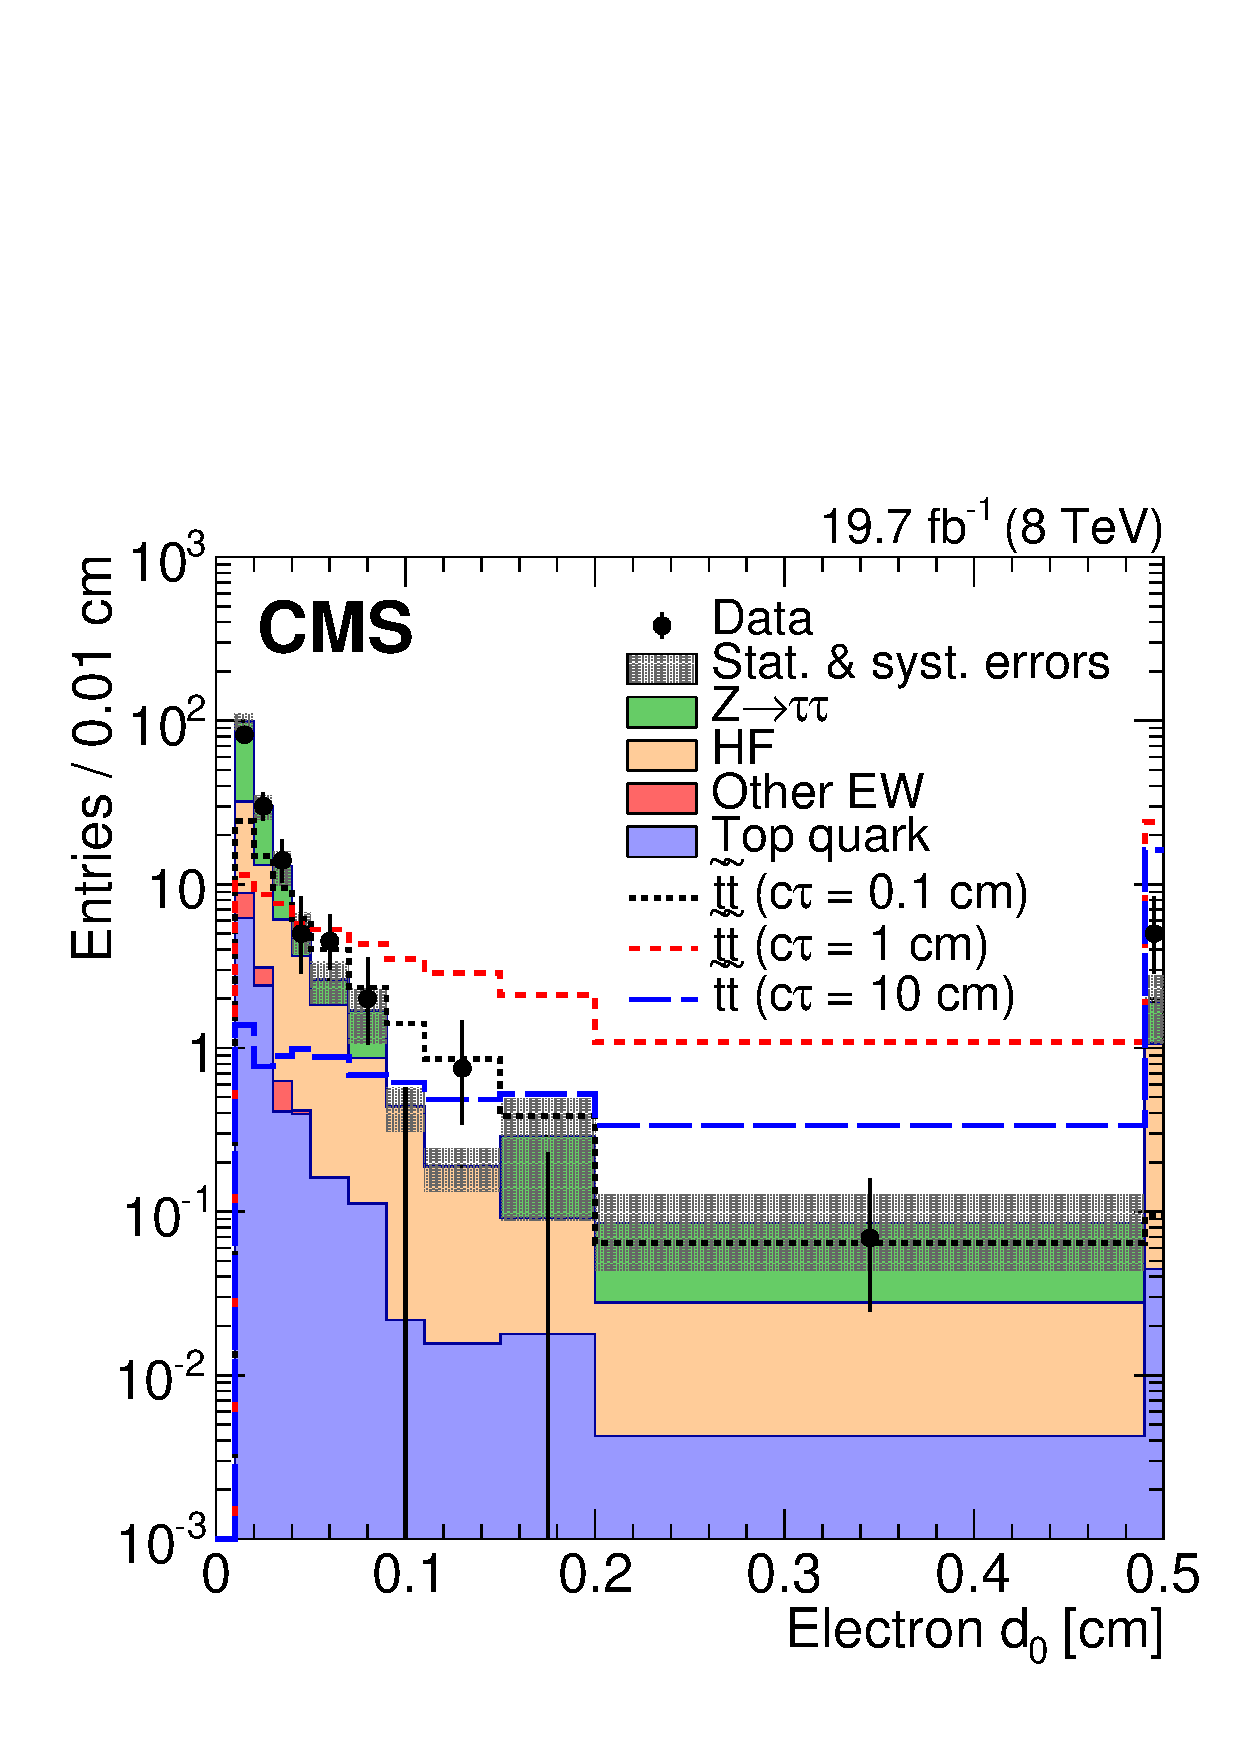
\includegraphics[height=3.0in]{CMS2015-bkg-e}
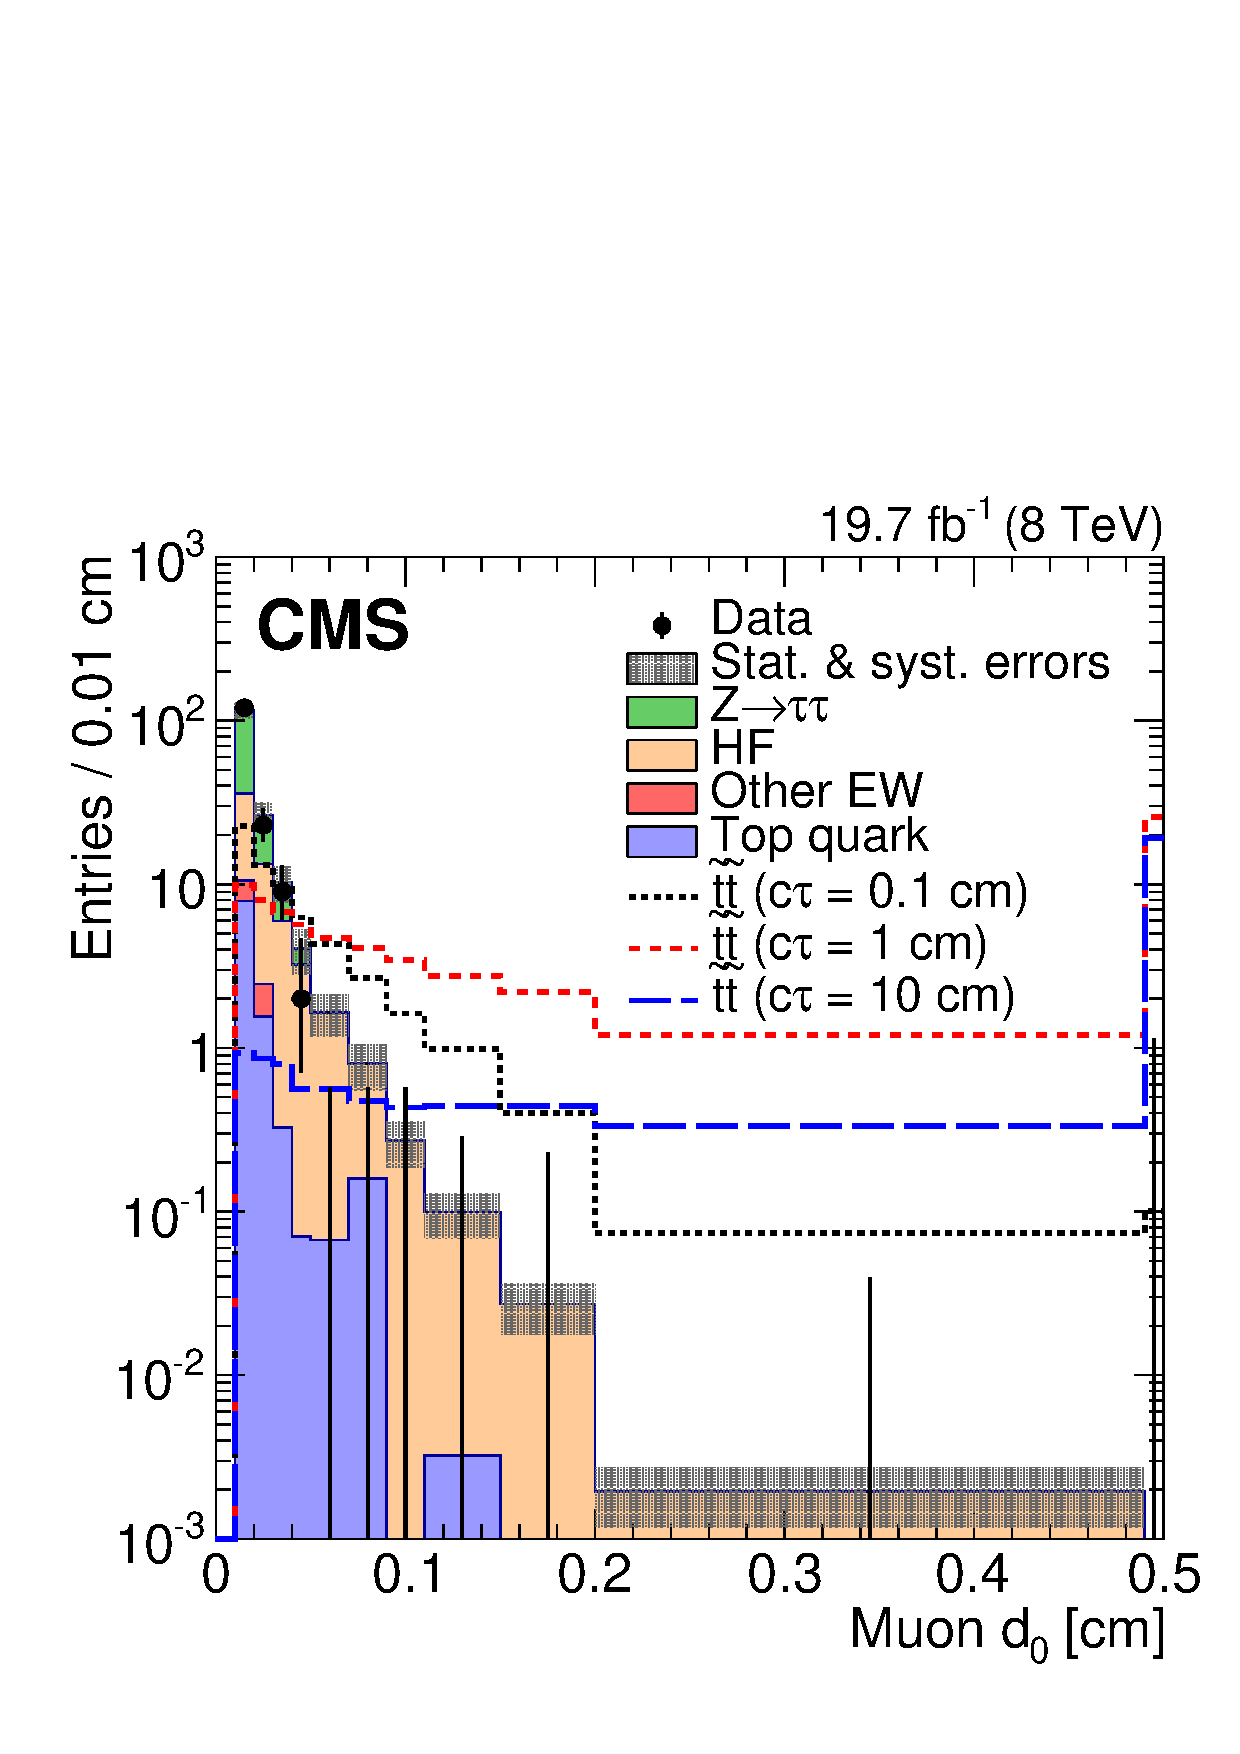
\includegraphics[height=3.0in]{CMS2015-bkg-mu}
\caption{\label{fig:CMS2015-bkg} Backgrounds from \cite{Khachatryan:2014mea}}
\end{figure}

\item 2016 CMS $e-\mu$-search for the opposite sign leptons with $d_0= 200 \text{ \mu m} -
10 \text{ cm}$, $\c \tau_{\tilde{t}}=10^{-2}-10^2 \text{ cm}$ \cite{CMS:2016isf}: decays of τ leptons and B or D mesons
with $c \tau_\tau \simeq 87 \text{ \mu m} ,\ c \tau_B \simeq 500 \text{ \mu m},\ c \tau_D \leq 100 \text{ \mu m}$ (Fig. \ref{fig:CMS2016-bkg}).

\begin{figure}[H]
\centering
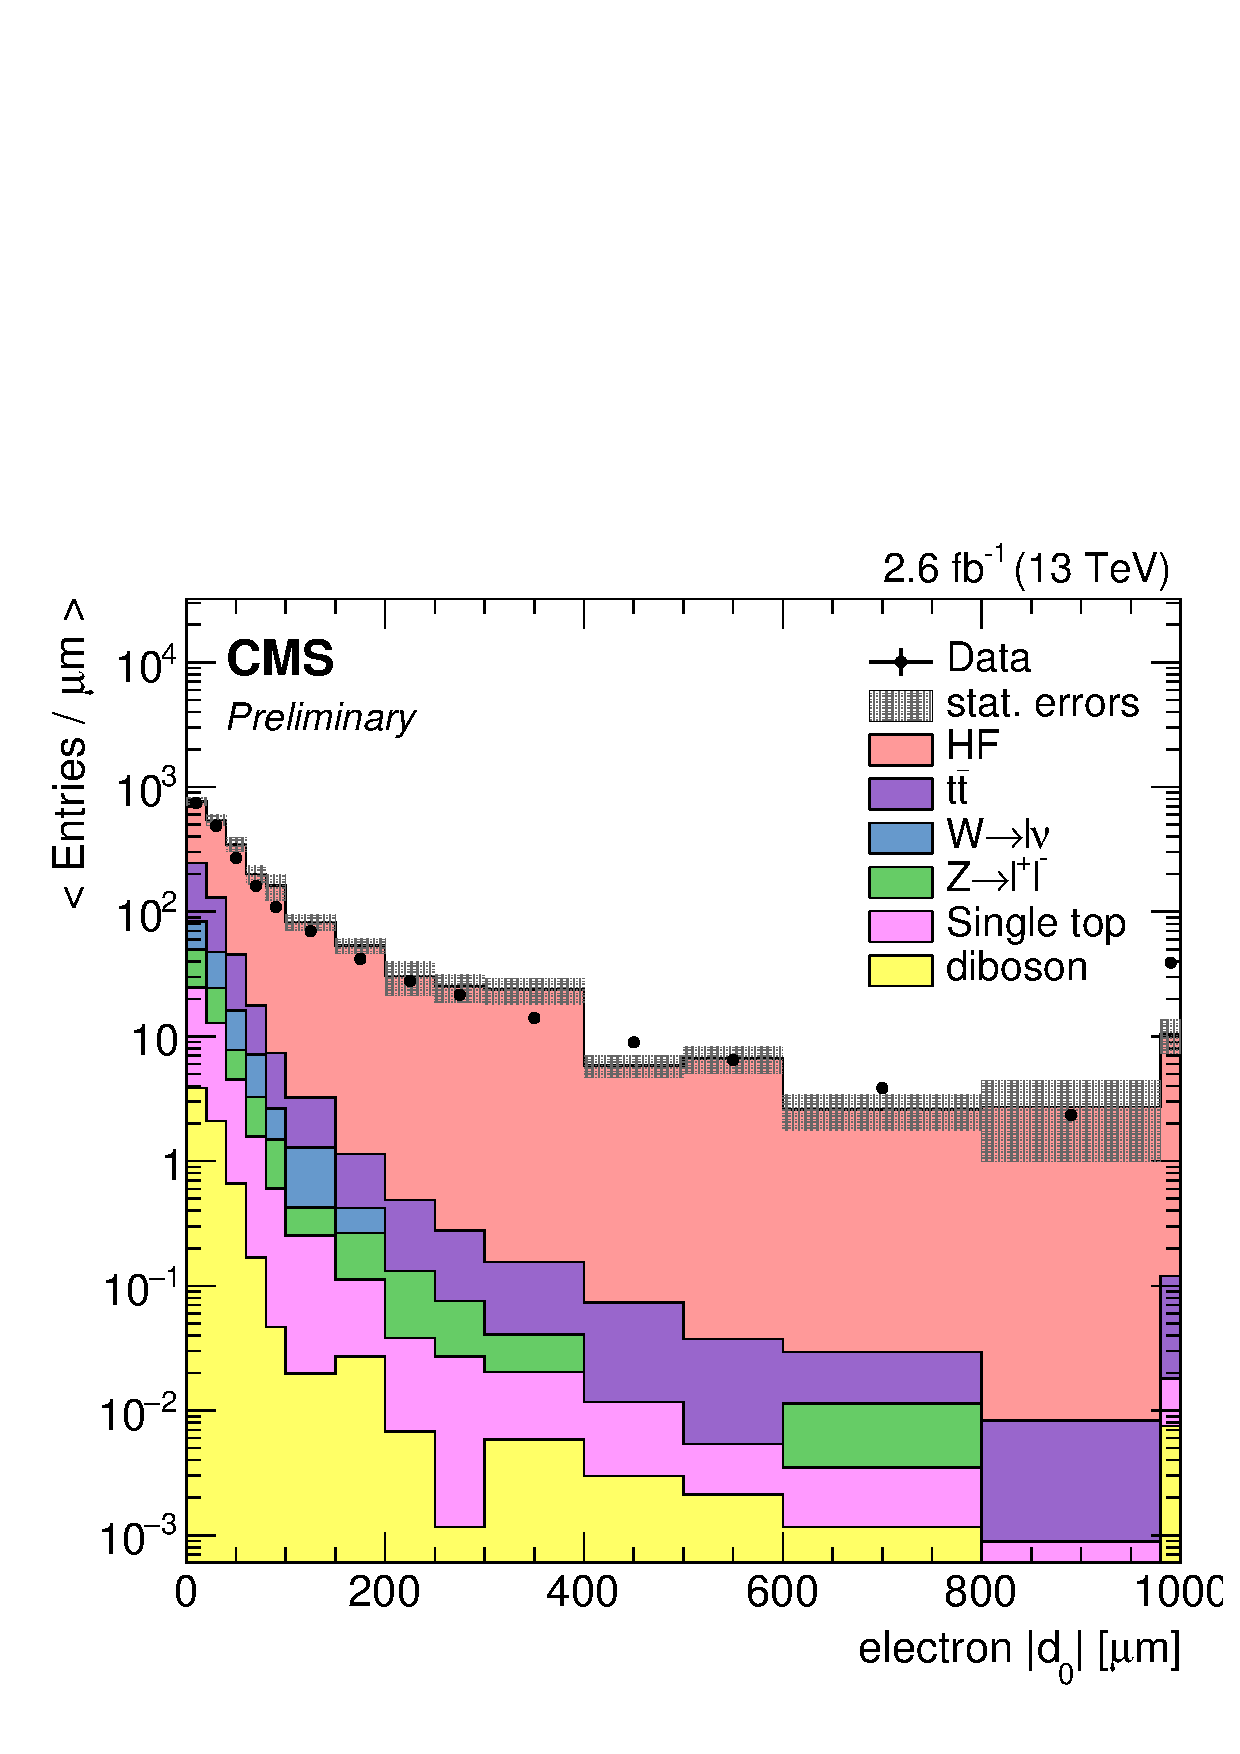
\includegraphics[height=3.0in]{CMS2016-bkg-e}
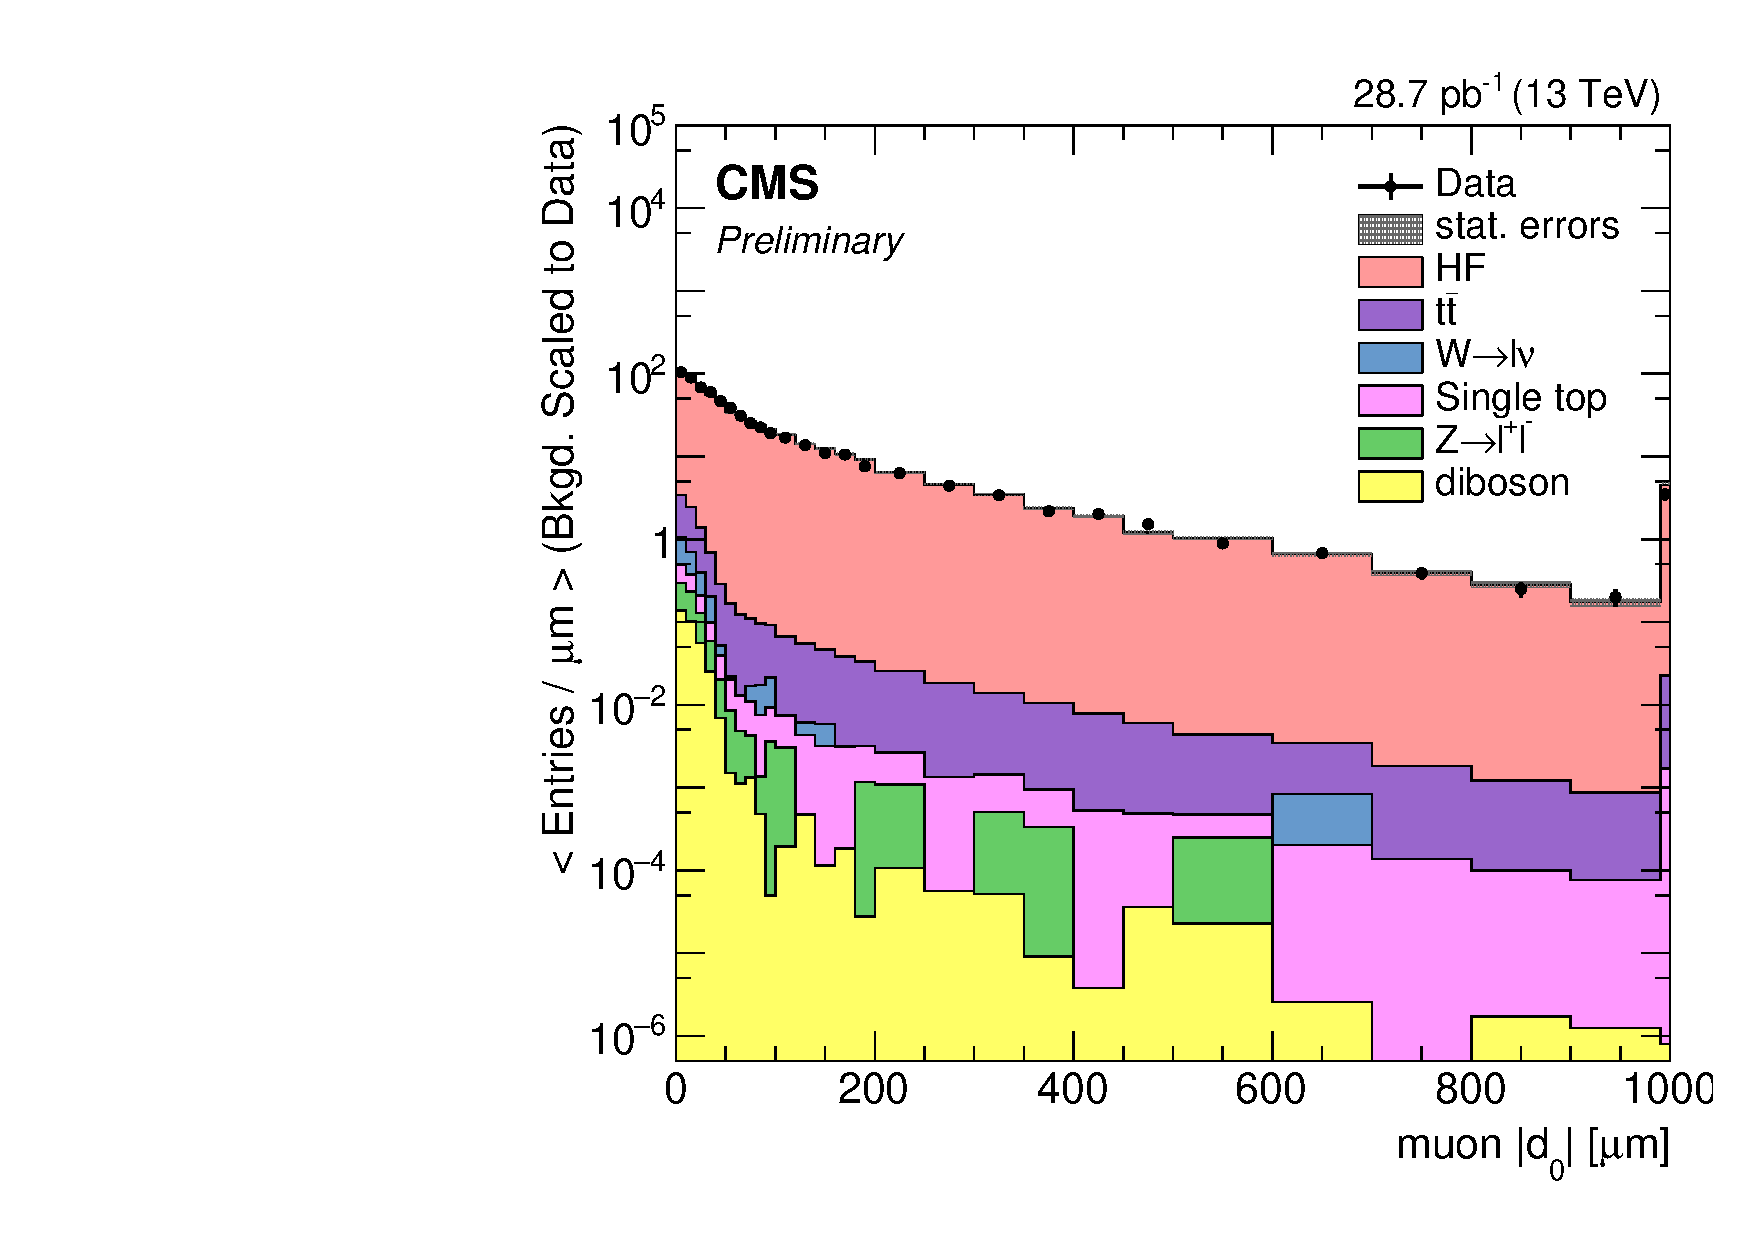
\includegraphics[height=3.0in]{CMS2016-bkg-mu}
\caption{\label{fig:CMS2016-bkg} Backgrounds from \cite{CMS:2016isf}}
\end{figure}

\item 208 CMS soft prompt oppositely charged (e or $\mu$) leptons \cite{Sirunyan:2018iwl}: ``The main backgrounds arise from events in which one of the leptons is not prompt (mainly
from W+jets events), events from fully leptonic tt decays ($t\bar{t}(2l)$), and Drell–Yan (DY) processes with subsequent decays $\gamma/Z^* \rightarrow \tau \tau \rightarrow ll \nu_l \nu_l \nu_\tau \nu_\tau$. Smaller backgrounds are from tW production (tW) and the diboson processes WW and $ZZ^*$, with $Z^* \rightarrow ll$ and $Z → \nu \nu$ (VV). Processes
such as $t\bar{t}W,\ t\bar{t}Z, WWW, ZZZ, WZZ$ and WWZ as well as processes including the Higgs boson have very small contributions, and are grouped together as “Rare”. ''

\end{itemize}

\begin{figure}[H]
\centering
\includegraphics[height=3.0in]{displaced-leptons.png}
\caption{\label{fig:2displaced_diagram}New signature of two displaced soft leptons at the LHC.}
\end{figure}

\subsection{Kinematics}

Here I list some kinematic properties of the process considered for 3 benchmark points that give the correct relic abundance. I consider only the scalar scenario because the kinematics depends only on the mass splittings wich are almost the same for both scenarios (however, once we'll be taking into account also the lifetimes, we should take care of both scenarios separately):

\begin{itemize}
  \item {\textbf BP \#1}: $m_l = 101 \text{ GeV},\ m_C = 114\text{ GeV}$
  \item {\textbf BP \#3}: $m_l = 300 \text{ GeV},\ m_C = 324 \text{ GeV}$
  \item {\textbf BP \#2}: $m_l = 500 \text{ GeV},\ m_C = 528 \text{ GeV}$
\end{itemize} \label{benchmarks_scalar}

The corresponding kinematic distributions for an example case of two displaced muons are plotted on Fig.\ref{fig:pT-eta},\ref{fig:inv_mass-PT_miss}. The distributions are expected to be the same also for the one displaced and one prompt lepton in final state.

\begin{figure}[H]
\centering

\includegraphics[height=1.4in]{figs/BP1_selection_0}
\includegraphics[height=1.4in]{figs/BP2_selection_0}
\includegraphics[height=1.4in]{figs/BP3_selection_0}

\includegraphics[height=1.4in]{figs/BP1_selection_1}
\includegraphics[height=1.4in]{figs/BP2_selection_1}
\includegraphics[height=1.4in]{figs/BP3_selection_1}

\includegraphics[height=1.4in]{figs/BP1_selection_4}
\includegraphics[height=1.4in]{figs/BP2_selection_4}
\includegraphics[height=1.4in]{figs/BP3_selection_4}

\includegraphics[height=1.4in]{figs/BP1_selection_5}
\includegraphics[height=1.4in]{figs/BP2_selection_5}
\includegraphics[height=1.4in]{figs/BP3_selection_5}


\caption{\label{fig:pT-eta} PT of leading muon (first row) and next-to-leading muon (second row); pseudorapidity of leading muon (third row) and next-to-leading muon (fourth row) for the benckmark point BP \#1,2,3 (from left to right). }
\end{figure}

\begin{figure}[H]
\centering


\includegraphics[height=1.4in]{figs/BP1_selection_10}
\includegraphics[height=1.4in]{figs/BP2_selection_10}
\includegraphics[height=1.4in]{figs/BP3_selection_10}

\includegraphics[height=1.4in]{figs/BP1_selection_12}
\includegraphics[height=1.4in]{figs/BP2_selection_12}
\includegraphics[height=1.4in]{figs/BP3_selection_12}

\includegraphics[height=1.4in]{figs/BP1_selection_15}
\includegraphics[height=1.4in]{figs/BP2_selection_15}
\includegraphics[height=1.4in]{figs/BP3_selection_15}


\caption{\label{fig:inv_mass-PT_miss} Invariant mass of the two oppositely charged muons (first row), $\Delta R$ of two oppositely charged muons (second row), missing transverse momentum (third row) for the benckmark point BP \#1,2,3 (from left to right). }
\end{figure}

\section{One displaced and one prompt lepton}

The production goes trough W-boson, leading to a signature with one displaced and one prompt lepton of the same or opposite signs (\ref{fig:2displaced_diagram}). The displacement on the long-branch side is caused by the mass splitting suppression $\Delta m_{hc} = m_h - m_c \approx \mu^2/(m_T - m_S) - 160\,\text{MeV}$ .~\footnote{Caution: this approximate formula is valid only in the small $\mu$ regime, however, $\mu$ is sizeable in the considered case} (we expect pion to be very soft, so that it is not observed), the second branch is prompt due to a relatively large mixing angle. The mass splitting between the charged and the light neutral states is again $\Delta m_{c \ell} = 15-30 \text{ GeV}$, and between the heavy neutral and the charge states: $\Delta m_{h c} \simeq 160 \text{ MeV}$. The lifetime of the charged state varies in the range $\c \tau_+ \simeq 0-0.5 \text{ cm}$ and the portal couplings $\mu/v \sim 10^{-2}\ (3\times 10^{-2}-10^{-1})$ in the scalar (pseudo-scalar) model.

\subsection{Expexted backgrounds}
Only non-symmetric processes:
\begin{itemize}
  \item W+jets events (?)
\end{itemize}

\begin{figure}[H]
\centering
\includegraphics[height=3.0in]{displaced+prompt-leptons.png}
\caption{\label{fig:2displaced_diagram}New signature of one displaced and one prompt soft leptons at the LHC.}
\end{figure}

\begin{thebibliography}{6}

\bibitem{Filimonova:2018qdc}
  A.~Filimonova and S.~Westhoff,
  %``Long live the Higgs portal!,''
  arXiv:1812.04628 [hep-ph].
  %%CITATION = ARXIV:1812.04628;%%

  \bibitem{Khachatryan:2014mea}
    V.~Khachatryan {\it et al.} [CMS Collaboration],
    %``Search for Displaced Supersymmetry in events with an electron and a muon with large impact parameters,''
    Phys.\ Rev.\ Lett.\  {\bf 114}, no. 6, 061801 (2015)
    doi:10.1103/PhysRevLett.114.061801
    [arXiv:1409.4789 [hep-ex]].


  \bibitem{CMS:2016isf}
    CMS Collaboration [CMS Collaboration],
    %``Search for displaced leptons in the e-mu channel,''
    CMS-PAS-EXO-16-022.

\bibitem{Sirunyan:2018iwl}
  A.~M.~Sirunyan {\it et al.} [CMS Collaboration],
  %``Search for new physics in events with two soft oppositely charged leptons and missing transverse momentum in proton-proton collisions at $\sqrt{s}=$ 13 TeV,''
  Phys.\ Lett.\ B {\bf 782}, 440 (2018)
  doi:10.1016/j.physletb.2018.05.062
  [arXiv:1801.01846 [hep-ex]].

\end{thebibliography}

\end{document}
